\chapter{Praxis}

Im folgenden wird die praktische Umsetzung der vorher erarbeiteten Theorie behandelt.
Hierzu wurde/wird ein Tool geschrieben, das aufgrund eines GraphQL-Schemas automatisiert Tests erzeugt.
Diese Tests werden dann ausgeführt und ausgewertet mit den entsprechenden Verbesserungen.

\section{Toolchain}

Da GraphQL ein Standard für diverse Sprachen ist und das "mocken" von Daten essentiell zum testen ist, kann
der Teil der Testgenerierung und Auswertung nur sprachspezifisch stattfinden. Es können somit nicht alle
Sprachen berücksichtigt werden.
Da GraphQL vor allem in der Webentwicklung verwendet wird, bezieht sich das Testtool auf JavaScript/TypeScript
mit der Testbibliothek Jest.
Als Server für die Verarbeitung wird ApolloServer genutzt, es ist jedoch denkbar,
dass man jeden Server einsetzen kann insofern dieser eine executeOperation() implementiert die einen
String als Query akzeptiert.
Um Daten zu generieren wird auf das Tool Factory.ts zurückgegriffen (kann sich noch ändern), dieses
ermöglicht es "Baupläne" anzulegen und dann beliebig viele Objekte zu erschaffen.
Die benötigte Toolchain ist also sehr klein, sie benötigt nur Factory.ts für die Datengenerierung,
Jest für die Ausführung der generierten Tests und
ApolloServer für die Ausführung der GraphQL-Resolver.

\section{Ablauf der Generierung}

\begin{center}
    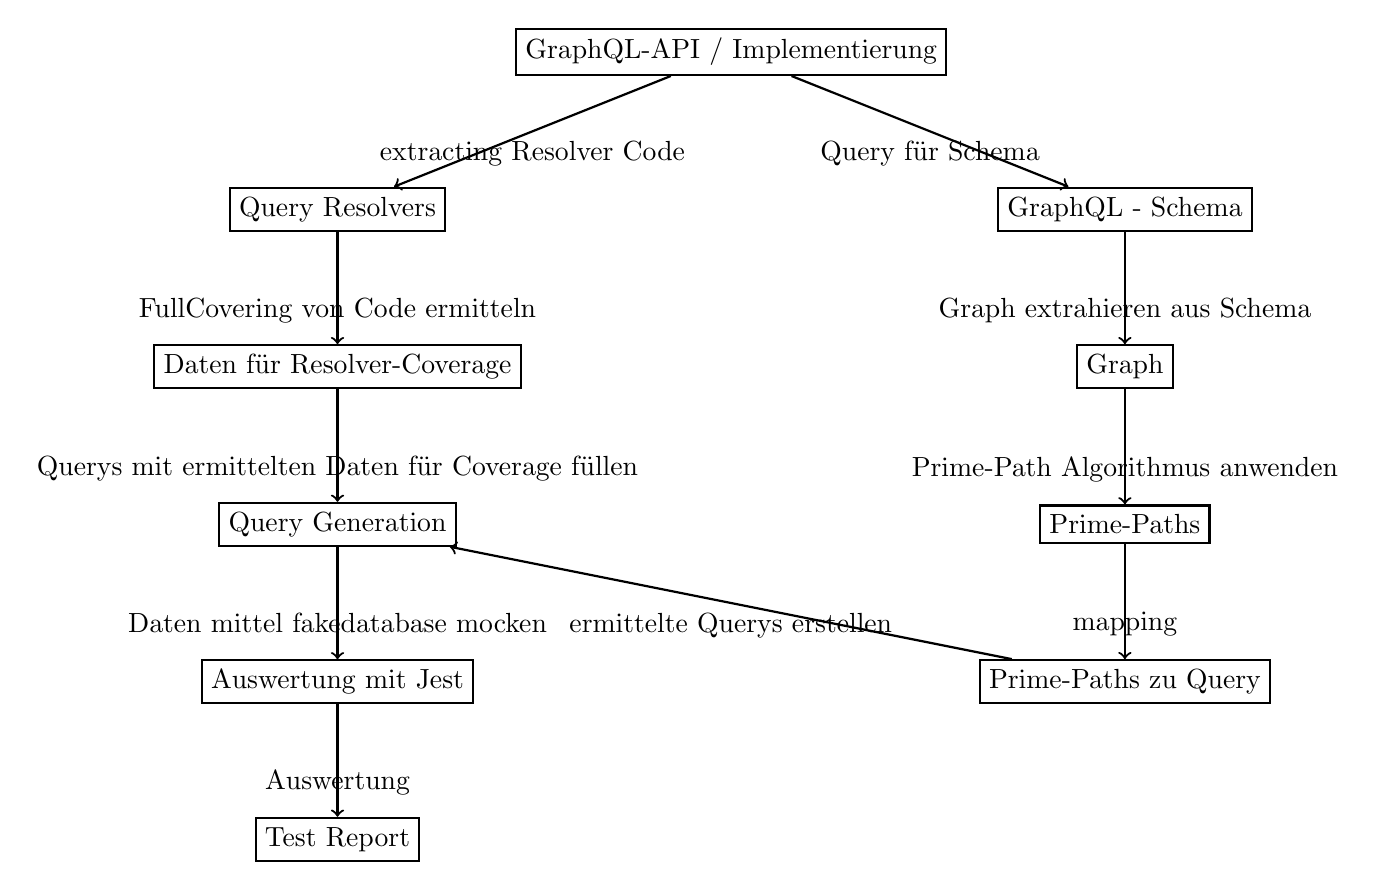
\begin{tikzpicture}[node distance={15mm}, thick, main/.style = {draw}]
        \node[main] at (5,10) (1) { GraphQL-API / Implementierung };
        \node[main] at (0,8) (2) { Query Resolvers };
        \node[main] at (10,8) (3) { GraphQL - Schema};
        \node[main] at (10,6) (4) { Graph };
        \node[main] at (10,4) (5) { Prime-Paths };
        \node[main] at (10,2) (6) { Prime-Paths zu Query };
        \node[main] at (0,6) (8) { Daten für Resolver-Coverage };
        \node[main] at (0,4) (9) { Query Generation };
        \node[main] at (0,2) (10) { Auswertung mit Jest };
        \node[main] at (0,0) (11) { Test Report };
        \draw [->] (1) to node [midway,below]{ Query für Schema } (3);
        \draw [->] (1) to node [midway,below]{ extracting Resolver Code } (2);
        \draw [->] (3) to node [midway,below]{ Graph extrahieren aus Schema } (4);
        \draw [->] (4) to node [midway,below]{ Prime-Path Algorithmus anwenden } (5);
        \draw [->] (5) to node [midway,below]{ mapping } (6);
        \draw [->] (2) to node [midway,below]{ FullCovering von Code ermitteln } (8);
        \draw [->] (8) to node [midway,below]{ Querys mit ermittelten Daten für Coverage füllen } (9);
        \draw [->] (6) to node [midway,below]{ ermittelte Querys erstellen } (9);
        \draw [->] (9) to node [midway,below]{ Daten mittel fakedatabase mocken } (10);
        \draw [->] (10) to node [midway,below]{ Auswertung } (11);
    \end{tikzpicture}
\end{center}


\section{Requirements an das Tool}

